\begin{table}[H]
\centering\small
\caption{Foundation architectures and completed training counters. FFN is the intermediate feed-forward width; contexts are architecture limits. Processed tokens count repeated training exposure, not unique corpus tokens.}
\label{tab:foundations}
\begin{tabular}{clrrrrr}
\toprule
Base & Family & Layers & Width / heads & FFN & Context & Params (M)\\
\midrule
01 & Causal & 8 & 768 / 12 & 2048 & 1024 & 82.012\\
02 & Encoder--decoder & 6+6 & 512 / 8 & 2048 & 1024/512 & 61.343\\
03 & Prefix hybrid & 24 & 384 / 6 & 1024 & 1280 & 52.206\\
04 & Local/global causal & 14 & 512 / 8Q:2KV & 1536 & 1536 & 55.113\\
\bottomrule
\end{tabular}
\end{table}

All four models minimize target cross-entropy, with held-out documents, tied embeddings and equal-probability source draws. Bases~01--04 completed 12k, 12k, 10k and 15k steps, processing 74.41M, 242.87M, 203.01M and 304.58M tokens. Base~04 combines a 256-token local window with a global anchor every 128 positions. Submission generation uses greedy cached decoding with a 128-word target. Since the runs differ in corpus subset, tokenizer and objective, their losses are not a controlled comparison of architecture alone.

\begin{figure}[H]
\centering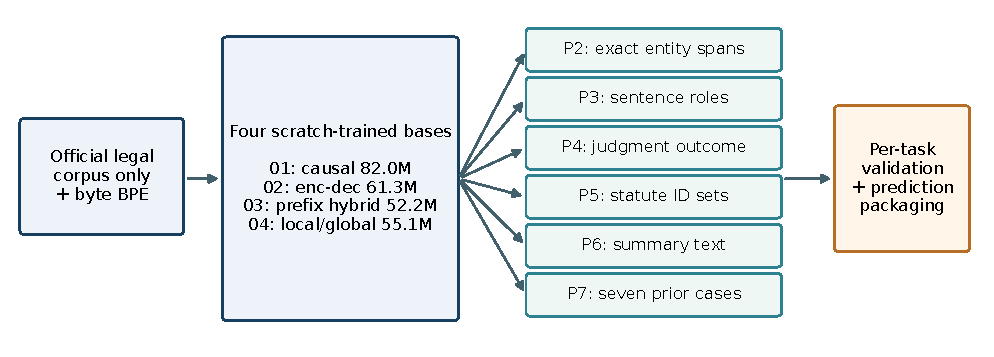
\includegraphics[width=\textwidth]{figures/architecture.pdf}
\caption{Actual transfer structure. Each downstream phase starts from an original foundation and trains its own head or adaptation. The tasks are separate descendants, rather than a seven-stage inference cascade.}
\end{figure}

\subsection{Transfer protocol (Phases 2--7)}
The downstream experiments vary how much of the foundation model is updated. Full tuning changes the backbone, while partial tuning changes only upper blocks. LoRA adds a low-rank update~\cite{hu2021lora}; LoRMA instead applies an identity-initialized multiplicative transformation to a frozen matrix~\cite{bihany2025lorma}. Other variants use bottleneck adapters~\cite{houlsby2019adapters}, activation scales~\cite{liu2022ia3} or soft prompts~\cite{lester2021prompt}. The adaptive-rank modules use an importance-based masking schedule inspired by AdaLoRA~\cite{zhang2023adalora}, rather than an exact reproduction of it. Distillation uses a teacher trained only on fitting data~\cite{hinton2015distill}. The README records the base and method for every slot.

\subsection{Phase 2 - Legal NER}
The first six NER methods use BIOUL tagging followed by character-boundary refinement. Later versions score span starts, ends and pairs directly in 384-token windows, with stride 288 and a 64-token span limit. V2 adds residual refinement and upper-layer tuning. V3 starts from V2, adds multiplicative start/end interactions and a residual pair network, and unfreezes twelve upper blocks. The final decoder selects a candidate source for each label from the raw and reranked V2/V3 outputs, then resolves overlaps and restores character offsets. Three document folds guide checkpoint and threshold selection. The reason for moving toward span extraction was practical: no threshold can recover a correct span that the candidate generator never proposes.
